\documentclass[../../../main.tex]{subfiles}

\begin{document}

\chapter{Data Structures}

So far, we discussed out C++ syntax, basic data structure, and
brute forcing some of the problems. In this note, we are going to
discuss about data structures. Learning data structures is not only
important in competitive programming but also in computer science
in general. Learning how to handle data more efficiently will make
us better programmers, so let's get right into it! Also, one more
thing. This note is largely based on the video ``Data Structures -
Full Course Using C and C++'' by Harsha and Animese \cite{CS02-9}.

\section{Lists and Linked Lists}

The first data structures that we are going to discuss are lists
and linked lists. Now we went over lists briefly before when we
discussed about arrays, but we haven't really gotten into how
arrays work under the hood. But before we get started, we need to
understand how memory is stored in RAM, what a memory address is,
and what a pointer is. I wrote a section specifically on that in
Section \ref{sec:26sbpfz}, so if you are unfamiliar with these topics,
please read that section first!

As always, let's get started with definition.

\begin{definition}{}{}
A \textbf{data structure} is a method for efficiently storing and
using data.
\end{definition}

So an example would be arrays. We used array to store some list of
data. Also when we say data structures, there are two main things:
Abstract Data Types (ADT) and implementation. But we will usually
refer to ADT, which defines the behavior of data structure and how
we use it without revealing underlying implementation of them.
Again, list is an exmple of ADT where arrays and linked list would
be implementation.

Okay, now on to lists and linked list. So what is a list? An example
of a list would be array. We could store, write, and read elements
given a position. Array is a list because say we have array
\verb|A|. We can access to read/write/modify elements in \verb|A| by
using its index like \verb|A[10]|. This is basically what list do!

\begin{figure}[H]
\centering
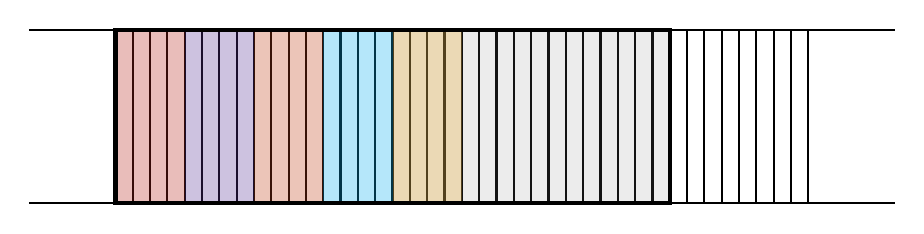
\begin{tikzpicture}[scale=1.1]
    \draw[thick] (0,1) -- (10,1);
    \draw[thick] (0,-1) -- (10,-1);
    \foreach \i in {1, 1.2, 1.4, ..., 8.8, 9} {
        \draw[thick] (\i,1) -- (\i,-1);
    }

    \fill[BrickRed, fill opacity=0.3] (1,1) rectangle (1.8,-1);
    \fill[RoyalPurple, fill opacity=0.3] (1.8,1) rectangle (2.6,-1);
    \fill[Bittersweet, fill opacity=0.3] (2.6,1) rectangle (3.4,-1);
    \fill[ProcessBlue, fill opacity=0.3] (3.4,1) rectangle (4.2,-1);
    \fill[Dandelion, fill opacity=0.3] (4.2,1) rectangle (5,-1);
    \fill[gray, fill opacity = 0.15] (4.2,1) rectangle (7.4,-1);
    \draw[ultra thick] (1,1) rectangle (7.4,-1);
\end{tikzpicture}
\end{figure}

Now list is very powerful when we know how many elements we have
and we know exactly how much memory we would need. But what about
the case when we don't know it? Usually when we define array in
C and C++, the \textbf{allocator} reserves consecutive slots in
RAM for the array. In other words if we run out of slot because
we need more elements, the allocator should reserve new slots
with more consecutive blocks and copy all the previous elements.

What about time complexity? If we want to insert, remove, or add
any element in a list, the worst case scenario would be to
travel all elements in the list to the place we want, so the
time complexity would be $\mathcal{O}(n)$. And by the nature of
lists, accessing would be constant time.

But again lists are good when we know exactly how many elements
we have, but it's not the best if we don't know. Creating a new
list and copying everything from before is very inefficient. This is
where linked list comes in! Well, there are other alternatives as
well, but let's focus on linked list for now.

Linked list is basically a list whose slots are not necessary
consecutive in memory. And theses slots are linked with pointers.
So say we we need to store an integer value. The allocator will
allocate $4$ bytes of memory for the integer and next $4$ or
$8$ bytes for pointer to the next element in the list. Then,
the next element will have a value and a pointer to the next element
in the list. The last element will have a value and $0$ because
no pointer that points to an existing memory address is zero and it
tells the linked list that it is is the last element. So basically,
linked list is a list that is connected through pointers.

\begin{figure}[H]
\centering
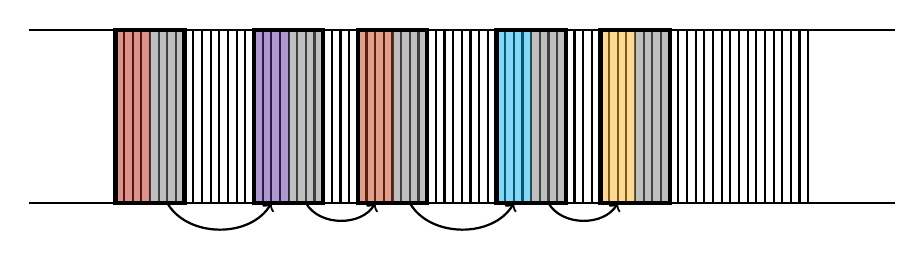
\begin{tikzpicture}[scale=1.1]
    \draw[thick] (0,1) -- (10,1);
    \draw[thick] (0,-1) -- (10,-1);
    \foreach \i in {1, 1.1, 1.2, ..., 8.9, 9} {
        \draw[thick] (\i,1) -- (\i,-1);
    }

    \fill[BrickRed, fill opacity=0.5] (1,1) rectangle (1.4,-1);
    \fill[Gray, fill opacity=0.5] (1.4,1) rectangle (1.8,-1);
    \draw[ultra thick] (1,1) rectangle (1.8,-1);

    \fill[RoyalPurple, fill opacity=0.5] (2.6,1) rectangle (3.0,-1);
    \fill[Gray, fill opacity=0.5] (3.0,1) rectangle (3.4,-1);
    \draw[ultra thick] (2.6,1) rectangle (3.4,-1);

    \fill[Bittersweet, fill opacity=0.5] (3.8,1) rectangle (4.2,-1);
    \fill[Gray, fill opacity=0.5] (4.2,1) rectangle (4.6,-1);
    \draw[ultra thick] (3.8,1) rectangle (4.6,-1);

    \fill[ProcessBlue, fill opacity=0.5] (5.4,1) rectangle (5.8,-1);
    \fill[Gray, fill opacity=0.5] (5.8,1) rectangle (6.2,-1);
    \draw[ultra thick] (5.4,1) rectangle (6.2,-1);

    \fill[Dandelion, fill opacity=0.5] (6.6,1) rectangle (7.0,-1);
    \fill[Gray, fill opacity=0.5] (7.0,1) rectangle (7.4,-1);
    \draw[ultra thick] (6.6,1) rectangle (7.4,-1);

    \draw[->, thick] (1.6,-1) to[bend right=60] (2.8,-1);
    \draw[->, thick] (3.2,-1) to[bend right=60] (4.0,-1);
    \draw[->, thick] (4.4,-1) to[bend right=60] (5.6,-1);
    \draw[->, thick] (6.0,-1) to[bend right=60] (6.8,-1);
\end{tikzpicture}
\end{figure}

Now let's see time complexity for linked lists. Inserting and
accessing elements requires linear time because in the worst case
scenario, we have to go through every links. But for inserting
at the beginning, it is constant time because we only care about
the \textbf{head}.

Compared to lists like an array, accessing have worse time complexity.
Also, it is harder to use! But there are certainly cases when linked
list is better. We don't waste memory! Large arrays may sometimes be
unavailable because the slots are consecutive. Also, if we don't use
all slots, then we are basically wasting memory with fixed size.
But for linked lists, we don't waste any because request for what we
need and we have more flexibility because we are not requesting for
a large block. Now let's see how we can implement a linked list with
C++.

\begin{cppbox}{26sbqhf-01}{26sbqhf-01}
\begin{lstlisting}[style=cppstyle]
#include <iostream>

struct element {
    int val;
    element* ptr;
};

int main() {
    element* HEAD = new element();
    HEAD->val = 0;

    element* temp = HEAD;
    for (int i = 1; i < 10; i++) {
        element* current = new element;
        current->val = i;
        current->ptr = nullptr;

        temp->ptr = current;
        temp = current;
    }

    element* search = HEAD;
    while ((*search).ptr != nullptr) {
        std::cout << (*search).val << " ";
        search = search->ptr;
    }
    std::cout << (*search).val << "\n";

    return 0;
}
\end{lstlisting}
\end{cppbox}

I know this can look intimidating at first, but let's break this part
by part. First, we defined the struct \verb|element|, which is
literally an element in our linked list. Each element will contain
a value and a pointer that points to another struct \verb|element|.

Now, we will declare \verb|HEAD| to be the pointer to the first head
element declared with \verb|new element()|. We then give value $0$.
Next, we are going to do the same thing. We declare another pointer
variable \verb|temp|, but this time, its value is initially
\verb|HEAD|.

Inside the for loop, we declare new pointer \verb|element|
that contains the value \verb|i| and has a null pointer.
So every \verb|current| is the last element in our linked list.
Then, we will tell \verb|temp| that the next element succeeding it
is \verb|current|. Now, we are going to move the temp to the current
new element. With this, we declared our linked list!

Now we want to search and print it. It works the same as we did it
now. We are going to create another dummy pointer variable
\verb|search| and this is going to be the first element \verb|HEAD|.
Lastly, we print the last element by hand because while loop
excludes it. Compiling and running it, we get the expected result!

\begin{outputbox}
\begin{lstlisting}[style=basic]
0 1 2 3 4 5 6 7 8 9
\end{lstlisting}
\end{outputbox}





\end{document}


